% =========================================================================== %
% Yes. This is a document.

\documentclass[
	english,
	aspectratio=169,
	table
]{beamer}

% =========================================================================== %
% Theme
\usepackage{scrlfile}
	\ReplacePackage{beamerthemeSHUR}{./sty/beamerthemeSHUR}
	\ReplacePackage{beamerinnerthemefancy}{./sty/beamerinnerthemefancy}
	\ReplacePackage{beamerouterthemedecolines}{./sty/beamerouterthemedecolines}
	\ReplacePackage{beamercolorthemechameleon}{./sty/beamercolorthemechameleon}

\usetheme[
	pageofpages=/,
	bullet=circle,
	titleline=true,
	alternativetitlepage=true,
	watermark="",
	watermarkheight=0px,
	watermarkheightmult=0
	]
{SHUR}

% =========================================================================== %
% the usual stuff

\usepackage[utf8]{inputenc}
\usepackage[T1]{fontenc}
\usepackage{babel}
\usepackage{lmodern}
\usepackage{microtype}
\usepackage{csquotes}
\usepackage{xspace}

\usepackage{tabularx}
\usepackage{booktabs}
\usepackage{multirow}

\usepackage{color, colortbl}
\usepackage{xcolor}
	\definecolor{tabhighlight}{RGB}{230,240,255}

\usepackage{tabto}
\usepackage{setspace}

\usepackage{minted}
	\usemintedstyle{friendly}

\usepackage{tikz}
	\usetikzlibrary{positioning}
	\usetikzlibrary{matrix}
	\usetikzlibrary{shapes.geometric}
	\usetikzlibrary{backgrounds}
	\usetikzlibrary{calc}
	\usetikzlibrary{decorations.pathreplacing}
	\tikzstyle{every picture}+=[remember picture] 
\usepackage{adjustbox}

\usepackage{amsmath}
\usepackage{physics}

\usepackage[most]{tcolorbox}
	\tcbsetforeverylayer
		{colback=cyan!10!white,
		 colframe=cyan!75!black,
		 arc=0pt,
		 outer arc=0pt
		}
	\newtcolorbox{codebox}[1][Code]
		{colback=black!5!white,
		 colframe=blue!40!black,
		 title=#1,
		 leftupper=6mm
		}
	\newtcolorbox{cmdbox}[1][Command Line]
		{colback=black,
		 coltext=white,
		 fontupper=\ttfamily ,
		 colframe=blue!40!black,
		 title=#1,
		 outer arc=0pt
		}
	\newtcolorbox{warnbox}[1][Warning]
		{colback=black!5!white,
		 colframe=red!40!black,
		 title=#1
		}
	\newtcolorbox{hintbox}[1][Hint]
		{colback=black!5!white,
		 colframe=green!40!black,
		 title=#1
		}
	\newtcolorbox{defbox}[1][Code]
		{colback=cyan!10!white,
		 colframe=cyan!90!black,
		 title=#1
		}
	\newtcolorbox{recapbox}[1][Code]
		{colback=yellow!10!white,
		 colframe=yellow!90!black,
		 coltitle=black,
		 title=#1
		}
%==============================================================================%
% GLOBAL MACROS

\newcommand*{\zB}{e.\,g. }
\newcommand*{\ie}{i.\,e. }

\newcommand{\Thus}{\ensuremath{\Rightarrow}\xspace}
\newcommand{\thus}{\ensuremath{\rightarrow}\xspace}

\newcommand*{\tabcrlf}{\\ \midrule}			% actually still allows for optional argument

\newcommand*{\inPy}[1]{\mintinline{python}{#1}}

\newcommand*{\todo}[1]{{\color{red}TODO: #1}}
\newcommand*{\sfrac}[2]{\ensuremath{{}^{#1}/_{#2}}}

% =========================================================================== %

\author{Stefan Hartinger}
\title{Python for Scientists}
\subtitle{Part 20: Networking Basics}
\institute{Department of Just Some Dude Who Likes to Talk}
\date{Winter 2023/24}

% =========================================================================== %

\begin{document}
\newcommand{\rx}[1]{\texttt{"{\color{olive}#1}"}}
\newcommand{\match}[1]{{\color{blue}#1}}
\newcommand{\qtt}[1]{\texttt{"{#1}"}}

% =========================================================================== %

\begin{frame}[t,plain]
\titlepage
\end{frame}

% =========================================================================== %

\begin{frame}[fragile]{Networking Problems}
%
\begin{center}
\begin{columns}
\column{.45\linewidth}
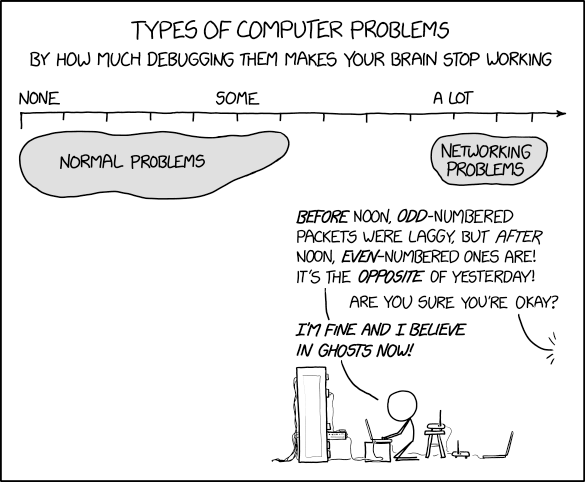
\includegraphics[width=\linewidth]{./gfx/20-xkcd-networking_problems}
%
\column{.45\linewidth}
\emph{LOOK, THE LATENCY FALLS EVERY TIME YOU CLAP YOUR HANDS AND SAY YOU BELIEVE}

\vspace{6pt}
Source: \url{https://xkcd.com/2259/}

\end{columns}
\end{center}
%
\end{frame}

% =========================================================================== %

\begin{frame}{Scope For Today}
%
\begin{itemize}
\item Network Jargon
	\begin{itemize}
	\item Protocols
	\item OSI Layers
	\item IP Adresses, Domains and Ports
	\item Networking in one machine
	\end{itemize}
\item Implementation in Python
	\begin{itemize}
	\item The \texttt{socket} package
	\item Multiplexing with the \texttt{select} package 
	\end{itemize}
\end{itemize}
%
\end{frame}

% =========================================================================== %

\begin{frame}{Protocols}
%
\begin{itemize}
\item Protocol: Standard for the \emph{order} and \emph{form} of messages
	\begin{itemize}
	\item Order: client sends username; server acknowledges; client sends password \emph{hash}, ...
	\item Form: usually header + payload
		\begin{itemize}
		\item E.\;g. integer (number of transferred bytes) plus some payload string
		\item Also: how does payload look like.
		\item E.\;g. string encoding, applied hash function, ...
		\end{itemize}
	\end{itemize}
\pause
\item Protocol execution may be more or less lenient
	\begin{itemize}
	\item E.\;g.: protocols may specify transferring additional error detection information
	\item If they are missing, communication could still be regarded as successfull.
	\item E.\;g.: protocol versions may differ; one party may send more information than the other one expects
	\item If the expected fields can be matches, communication could still be regarded as successfull.
	\end{itemize}
\end{itemize}
%
\end{frame}

% =========================================================================== %

\begin{frame}{OSI Layers}
%
\begin{itemize}
\item OSI: Open Systems Interconnection
	\begin{itemize}
	\item ISO Standard for responsibilities of networking protocols (meta-standard)
	\item Seven levels of abstraction (Layers)
		\begin{itemize}
		\item Higher layers make abstract requests
		\item Lower layers deal with the specifics
		\item Layer names: Physical, Data Link, Network, Transport, Session, Presentation, and Application
		\end{itemize}
	\end{itemize}
\pause
\item In practice: boundaries often blurred
	\begin{itemize}
	\item E.\;g.: Ethernet defines Layer 1+2 responsibilities
	\end{itemize}
\item[\Thus] Focus less on the boundaries between layers and more on the problems that must be solved for network communication
\pause
\item Not to be confused with the layers of the \emph{Internet Protocol Suite}
	\begin{itemize}
	\item Mostly the same; Missing layer 1, layers 5-7 merged into one, subtle differences
	\end{itemize}
\end{itemize}
%
\end{frame}

% =========================================================================== %

\begin{frame}{OSI Layers 1-2}
%
\begin{columns}
\column{.6\linewidth}
\begin{itemize}
\item Layer 1: Physical Layer
	\begin{itemize}
	\item Defines physical form of raw data
	\item The \enquote{form of bits}: voltages, light pulses, radio signals, ...
	\item Transmission rate, noise considerations
	\item Mostly Hardware
	\end{itemize}
\end{itemize}
%
\column{.3\linewidth}
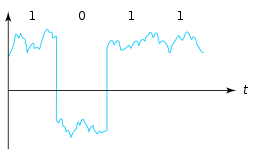
\includegraphics[width=\linewidth]{./gfx/20-Digital-signal-noise}
{\tiny \setstretch{1.0}
 \url{https://commons.wikimedia.org/wiki/File:Digital-signal-noise.svg}\\}
\end{columns}
\pause
%
\begin{itemize}
\item Layer 2: Data Link Layer
	\begin{itemize}
	\item Defines communication between \emph{two directly connected} machines
	\item Ensure Receiver is even listening
		\begin{itemize}
		\item E.\;g. send and wait for ACK
		\end{itemize}
	\item Format of messages
		\begin{itemize}
		\item E.\;g. Ethernet frame: sender and receiver MAC addresses, payload size; sync patterns
		\item Maximum message length
		\end{itemize}
	\item \emph{Some} data link protocols provide error correction mechanisms
		\begin{itemize}
		\item Checksums, requests for repetition
		\end{itemize}
	\end{itemize}
\end{itemize}
%
\end{frame}

% =========================================================================== %

\begin{frame}[fragile]{Layers 3-4}
%
\begin{columns}
\column{.7\linewidth}
\vspace{-9pt}
\begin{itemize}
\item Layer 3: Network Layer
	\begin{itemize}
	\item Defines communication \emph{over a network}
	\item End points need not be directly connected
	\item[\Thus] Primary objective: Routing, congestion prevention
	\item All nodes in the network have a unique \emph{address} 
	\item[\Thus] \zB IP-Addresses (\emph{Internet Protocoll}) 
	\end{itemize}
\end{itemize}
%
\column{.25\linewidth}
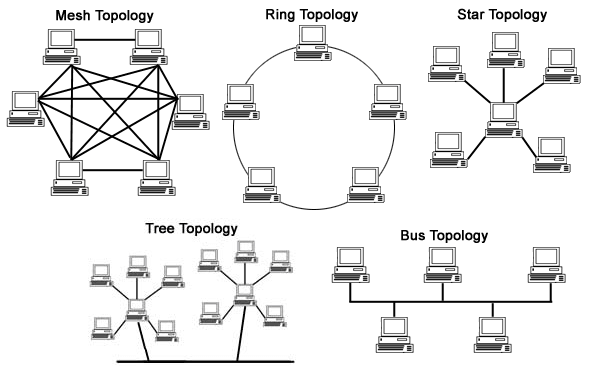
\includegraphics[width=\linewidth]{./gfx/20-network_topologies}
{\tiny \setstretch{1.0}
 \url{https://www.computerhope.com/jargon/n/network.htm}\\}
\end{columns}
\pause
%
\vspace{-9pt}
\begin{columns}
\column{.7\linewidth}
\begin{itemize}
\item Layer 4: Transport Layer
	\begin{itemize}
	\item Segmentation of large payloads to meet layer 2 needs
	\item Connection-oriented communication, reliability and multiplexing.
		\begin{itemize}
		\item Connection-oriented: Handshake before communication \\
			\Thus Ensures correct order of segments
		\item Reliability: Messages might get lost or get out of order \\
			\Thus repair mechanisms and requests to re-send
		\item Multiplexing: one \emph{host} might maintain multiple connections \\
			\Thus track context details
		\end{itemize}
	\end{itemize}
\end{itemize}
%
\column{.25\linewidth}
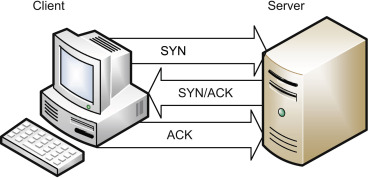
\includegraphics[width=\linewidth]{./gfx/20-tcp-handshake}
{\tiny \setstretch{1.0}
 \url{https://www.sciencedirect.com/topics/computer-science/three-way-handshake}\\}
\end{columns}
%
\end{frame}

% =========================================================================== %

\begin{frame}{Layers 5-6}
%
\begin{itemize}
\item Layer 5: Session Layer
	\begin{itemize}
	\item Session: exchange of multiple messages (groups of segements) between two machines belonging to a given context (\zB one website, one program)
	\item Might try to recover connection when temporarily lost
	\item Dialogue control, Timeouts, Synchronization
	\end{itemize}
\pause
\item Layer 6: Presentation Layer
	\begin{itemize}
	\item Translation of complex data into byte streams and back
	\item Serialization, byte order, string encoding
		\begin{itemize}
		\item XML, JSON
		\item UTF, ASCII, EBICDIC, Base64, ...
		\item C-Style (Null terminator) or Pascal Style (tuple of size and data)
		\item Endianness of Multi-Byte-Sequences
		\end{itemize}
	\end{itemize}
\end{itemize}
%
\end{frame}

% =========================================================================== %

\begin{frame}[fragile]{Layers 7-8}
%
\begin{itemize}
\item Layer 7: Applicaiton Layer
	\begin{itemize}
	\item Defines type and order of messages for a concrete use case
	\item[\Thus] Who sends what when, and what are appropriate responses to any given message
	\item Examples: 
		\begin{columns}
		\column{.4\linewidth}
			\begin{itemize}
			\item HTTP/HTTPS (Hypertext Transfer Protocol/Secure)
			\item FTP (File Transfer Protocol)
			\end{itemize}
		\column{.4\linewidth}
			\begin{itemize}
			\item SMTP (\emph{Simple Mail Transfer Protocol})
			\item SSH (Secure Shell)
			\end{itemize}
		\end{columns}
	\end{itemize}
\end{itemize}
\pause
%
\begin{hintbox}[OSI Layer 8]
\footnotesize
Sys-admins will sometimes identify some problems as \emph{Layer 8 problems}. Since the entity that makes requests to an application is usually a human, these problems often have the \enquote{error code} \emph{PEBKAC} (\enquote{Problem exists between keyboard and chair}).

For other extensions to the OSI model see \url{https://en.wikipedia.org/wiki/Layer_8}
\end{hintbox}
%
\end{frame}

% =========================================================================== %

\begin{frame}{Adresses}
%
\begin{itemize}
\item OSI Layer 3 Specification
	\begin{itemize}
	\item À priori any unique identifier; could be a string like \texttt{Stefan's Computer}
	\item Requirement: decomposability into subnet adresses: \texttt{Stefan, Regensburg, Germany}
		\begin{itemize}
		\item[\Thus] Enables more effficient routing. Cf. \url{https://xkcd.com/195/}
		\end{itemize}
	\item Numbers more advantageous, because uniform length
	\pause
	\end{itemize}
\item IP Addresses
	\begin{itemize}
	\item Commonly known IPv4 address: 32 bit number, usually denoted by four byte numbers
		\begin{itemize}
		\item Allows up to 4 billion addresses
		\item Private/Public addresses increase number of devices online at the same time
		\item Special addresses with fixed meanings
		\item E.\;g. \texttt{127.0.0.1} (aka localhost)
		\end{itemize}
	\pause
	\item Slowly replaced by IPv6: 128 bit number; implicit changes to the protocol
		\begin{itemize}
		\item Primarily allows more addresses \Thus more devices online (2023: ca. 10 billion devices online)
		\item Also some additions for broadcasting and security
		\item Form: eight groups of four hex digits, separated by colons
		\item Consecutive null sequences may be indicated by double colon
		\item E.\;g. \texttt{2001:0db8:{\color{blue}0000:0000:0000}:8a2e:0370:7334} aka \texttt{2001:db8{\color{blue}::}8a2e:370:7334}
		\end{itemize}
	\end{itemize}
\end{itemize}
%
\end{frame}

% =========================================================================== %

\begin{frame}{Ports}
%
\begin{itemize}
\item (IP-) address identifies machine (aka host), but not the \emph{context} at the target
	\begin{itemize}
	\item One machine might run several processes, each of which may maintain several connections
	\item E.\;g.: Web Browser with several tabs, music streaming app, email client
	\end{itemize}
\pause
\item[\Thus] Additional datum: Port
	\begin{itemize}
	\item Just a 16bit number (values 0 to 65535), defined in layer 4
	\item Think of it as a process ID
	\item Split in \emph{well-known}, \emph{registered} and \emph{dynamic/private/ephemeral} ports
		\begin{itemize}
		\item Well-known ports (0 to 1023): associated with specific services (\zB HTTP, SMTP, FTP)
		\item Registered ports (1024 to 49151): Commercial use
		\item Ephemeral ports (49152–65535): Free to use
		\item See \url{https://en.wikipedia.org/wiki/List_of_TCP_and_UDP_port_numbers}
		\end{itemize}
	\end{itemize}
\pause
\item OS implementation of layer 5 forwards incoming data to processes given a \emph{socket}
	\begin{itemize}
	\item A socket is uniquely defined by the tuple of tuples\\
		((sender-IP, sender-port), (receiver-IP, receiver-port))
	\end{itemize}
\end{itemize}
%
\end{frame}

% =========================================================================== %\\

\begin{frame}{Example: Web Browser}
%
\begin{itemize}
\item When loading a website, the following steps are performed
	\begin{itemize}
	\item Client selects an unused ephemeral port (eg. 60000)
	\item Client creates a socket for the communication with the HTTP server
		\begin{itemize}
		\item socket: ((\emph{client-IP}, \texttt{60000}), (\emph{server-IP}, \texttt{80}))
		\end{itemize}
\pause
	\item Client initiates handshake with server
		\begin{itemize}
		\item Client sends request to initiate communication
		\item Server replies with ok signal and creates its own socket
		\item Client responds with ok signal \Thus both parties know they can hear each other
		\end{itemize}
\pause
	\item HTTP communication itself is executed
		\begin{itemize}
		\item Client sends HTTP request
		\item Server sends website
		\item Client confirms correctly receiving the website
		\item Communication ends, both sockets are closed
		\end{itemize}
\pause
	\item Note
		\begin{itemize}
		\item Well-known port 80 associated with HTTP \Thus server knows what messages to expect
		\item Other hosts can still connect to server on same port, (client-tuple ensures correct routing)
		\item Connections on other ports are possible, too, but answered by other processes on server
		\end{itemize}
	\end{itemize}
\end{itemize}
%
\end{frame}

% =========================================================================== %

\begin{frame}{Domains and Name Servers}
%
\begin{itemize}
\item Numbers: good for computers, but not for humans \Thus Mapping: String to IP address
\item Done by DNS (\emph{domain name service}) servers
	\begin{itemize}
	\item Service specified by a OSI Layer 7 protocol
	\item Provided by a few well known static IP addresses
	\item E.\;g. \texttt{8.8.8.8} or \texttt{2001:4860:4860::8888}: Google DNS server
	\item Dozends of other DNS servers, free and premium versions, different speed and extra features like malware protection
	\end{itemize}
\pause
\item Domains themselves
	\begin{itemize}
	\item Strings separated into segments by dots
	\item Read back to front: \texttt{en.wikipedia.org}
		\begin{itemize}
		\item First evaluate \texttt{org}, aka TLD (\emph{top level domain})
		\item Subsequently resolve \emph{subdomains}, \ie \texttt{wikipedia} and finally \texttt{en}
		\end{itemize}
	\pause
	\item Prefixed by a \emph{protocol} indicator, e.\;g. \texttt{http://}, \texttt{https://}, \texttt{ftp://}, ...
	\pause
	\item May be followed by a path on the server
		\begin{itemize}
		\item Think of an actual file path \thus same notation
		\item \texttt{{\color{gray}https://en.wikipedia.org}/wiki/Subdomain}
		\end{itemize}
	\end{itemize}
\end{itemize}
%
\end{frame}

% =========================================================================== %

\begin{frame}{Python Package \texttt{socket}}
%
\begin{itemize}
\item Socket: \enquote{Low-level networking interface}: implements OSI Layer 4/5 interface
	\begin{itemize}
	\item Allows communication like in the web browser example
	\item Can interface with a large number of Layer 4 protocols, \zB TCP/IP, Bluetooth, CAN, ...
	\item My Ex-Girlfriend: \emph{a mixture between socks and rockets}
	\end{itemize}
\pause
\item Primary commands (server and client side)
	\begin{itemize}
		\item \texttt{socket} -- creates a \texttt{socket} for specified lower layer protocols
	\end{itemize}
	\vspace{-18pt}
	\begin{columns}[t]
	\column{.38\linewidth}
	\begin{itemize}
		\item \texttt{bind} -- server side, binds the \texttt{socket} to an address and port
		\item \texttt{listen} -- server side, registers incoming connection attempts
		\item \texttt{accept} -- server side, participates in the three-way handshake
	\end{itemize}
	\column{.38\linewidth}
	\begin{itemize}
		\item \texttt{connect} -- client side, attempts a three-way handshake with a server
	\end{itemize}
	\end{columns}
	\begin{itemize}
		\item \texttt{send} and \texttt{recv} -- send and receive \inPy{bytes} objects given a completed handshake
		\item \texttt{close} -- ends communication
	\end{itemize}
\end{itemize}
%
\end{frame}

% =========================================================================== %

\begin{frame}{Preparing a \texttt{socket} Object}
%
\inPy{socket.socket(family, type, protocol = 0)} returns a \texttt{socket} object
\begin{itemize}
\item \texttt{family} -- specifies address format (\zB IPv4, Bluetooth, ...)
	\begin{itemize}
	\item \texttt{AF\_INET} -- IPv4. Addreses are \texttt{(host, port)}
		\begin{itemize}
		\item \texttt{host}: a \inPy{str}ing specifying the target machine \\
			May be an IP address (\zB \inPy{'127.0.0.1'}) or a domain name (\zB \inPy{'en.wikipedia.org'})
		\item \texttt{port} is an \inPy{int}.
		\end{itemize}
	\item \texttt{AF\_INET6} -- IPv6. Addresses are \texttt{(host, port, flowinfo, scope\_id)}
		\begin{itemize}
		\item \texttt{host} and \texttt{port}: same as above (but different IP address format)
		\item \texttt{flowinfo}: optional 32bit integer, allows grouping messages from different sources into a shared context
		\item \texttt{scope\_id}: optional 32bit integer, specifying where the address is valid \\
			See \url{https://en.wikipedia.org/wiki/IPv6_address}
		\end{itemize}
	\item \texttt{AF\_BLUETOOTH} -- Bluetooth. Addresses have different formats depending on \texttt{protocol}
		\begin{itemize}
		\item Usually some form of \inPy{(str, int)} where the string is a six-byte address (\texttt{12:34:56:78:90:AB})
		\item See \url{https://docs.python.org/3/library/socket.html}
		\end{itemize}
	\end{itemize}
\end{itemize}
%
\end{frame}

% =========================================================================== %

\begin{frame}{Preparing a \texttt{socket} Object}
%
\inPy{socket.socket(family, type, protocol = 0)} returns a \texttt{socket} object
\begin{itemize}
\item \texttt{type} -- specifies the OSI Layer 4 protocol
	\begin{itemize}
	\item \texttt{SOCK\_STREAM} -- specifies TCP (\emph{Transmission Control Protocol}), which is probably what you want
		\begin{itemize}
		\item Reliability mechanism -- dropped or corrupted packages are re-transmitted
		\item In-order delivery -- Messages arrive in same order they are sent
		\end{itemize}
	\item \texttt{SOCK\_DGRAM} -- specifies UDP (\emph{User Datagram Protocol})
		\begin{itemize}
		\item Less overhead, less traffic
		\item Used \zB for webradios, DNS, Time servers, ...
		\end{itemize}
	\end{itemize}
\item \texttt{protocol} -- \texttt{int} constant needed only for some address families
	\begin{itemize}
	\item Cf. \texttt{AF\_BLUETOOTH}
	\end{itemize}
\end{itemize}
%
\begin{hintbox}[Local Naming Convention]
\footnotesize
Since \texttt{socket} already denotes the package and the class, instances of \texttt{socket} will be mentioned as \texttt{s} in this presentation.
\end{hintbox}
%
\end{frame}

% =========================================================================== %

\begin{frame}{Building Up a Connection -- Server Side}
%
\begin{itemize}
\item \texttt{s.bind(address)} -- set's the host side address
	\begin{itemize}
	\item \texttt{address} is one of the \inPy{tuple}s specified with the \texttt{family} parameter of \texttt{socket.socket}
	\item Specifies \emph{own} address, \ie how to reach this host
	\item Address string can be empty -- consider all incoming requests (on the specified port)
	\item This socket is \emph{not} capable of communication
	\item Only a filter which incoming connection requests to consider
	\end{itemize}
\pause
\item \texttt{s.listen(n)} -- waits for a client to connect
	\begin{itemize}
	\item Puts \texttt{s} into listening mode, \ie registers all incoming connection attempts
	\item Up to \texttt{n} incoming connections before it refuses them automatically
	\item \texttt{n} can be ommitted -- \enquote{reasonable default value}
	\end{itemize}
\pause
\item \texttt{s.accept()} -- accepts an incoming request from a client
	\begin{itemize}
	\item Blocking call -- program freezes until a client actually connects
	\item Can be made nonblocking (see later)
	\item Returns a \inPy{tuple (conn, address)}
	\item \texttt{address} is the client address, which is in turn the \inPy{tuple (ip, port)}
	\item \texttt{conn} is a \texttt{socket} object that \emph{can} be used to send and receive data
	\end{itemize}
\end{itemize}
%
\end{frame}

% =========================================================================== %

\begin{frame}{Client Side -- Connecting to Server and Picking a Port}
%
\begin{itemize}
\item Connect to a server
	\begin{itemize}
	\item \texttt{s.connect(address)}
		\begin{itemize}
		\item \texttt{address} is one of the \inPy{tuple}s specified with the \texttt{family} parameter of \texttt{socket.socket}
		\item After this, \texttt{s} is actually capable to send/receive data
		\item Does all the Layer 4 magic needed before exchanging messages
		\end{itemize}
	\end{itemize}
\pause
\item Picking a port
	\begin{itemize}
	\item Use \texttt{bind} with null arguments: \inPy{s.bind(('', 0))}
		\begin{itemize}
		\item Note the double parens -- \texttt{bind} takes a \inPy{tuple} argument!
		\end{itemize}
	\item \texttt{s.getsockname()} returns \inPy{tuple(ip_address, port_id)}
		\begin{itemize}
		\item \texttt{ip\_address} will be a null address (\zB \texttt{0.0.0.0})
		\item \texttt{port\_id} is chosen by OS and names an ephemeral port
		\end{itemize}
	\item This is done automatically by the \texttt{connect} method
	\end{itemize}
\end{itemize}
%
\end{frame}

% =========================================================================== %

\begin{frame}{Sending and Receiving Data (Both Ends)}
%
\begin{itemize}
\item \texttt{s.send(bytes\_data)}
	\begin{itemize}
	\item May be used after \texttt{s.accept()} (server side) or \texttt{s.connect()} (client side)
	\item Attempts to send \texttt{bytes\_data}
	\item Might only send a portion thereof, returns \texttt{number\_of\_sent\_bytes}
	\end{itemize}
\pause
\item \texttt{s.sendall(bytes\_data)}
	\begin{itemize}
	\item May be used after \texttt{s.accept()} (server side) or \texttt{s.connect()} (client side)
	\item Sends \texttt{bytes\_data}, possibly in several packets
	\item Returns \inPy{None}
	\item Uses (multiple calls to) \texttt{s.send()} under the hood
	\end{itemize}
\pause
\item \texttt{s.recv(max\_number\_of\_bytes)}
	\begin{itemize}
	\item May be used after \texttt{s.accept()} (server side) or \texttt{s.connect()} (client side)
	\item Waits for an incoming message, and accepts at most \texttt{max\_number\_of\_bytes} bytes.
	\item Returns a \inPy{bytes} object
	\end{itemize}
\end{itemize}
%
\end{frame}

% =========================================================================== %

\begin{frame}
%
\vspace{-6pt}
\begin{hintbox}[Stream-Based Protocol]
\footnotesize
Unfortunately, there is no mechanism in TCP that marks begin or end of a message.

If you send two messages comprising four bytes each, and attempt to receive up to eight bytes, you will get both messages in one go.
This means you have to define your own \emph{message exchange protocol} on top of TCP. 

Usually this simply means you prepend a header containing the message length in bytes to your actual payload.
With this, the receiving side can first \texttt{recv(size\_of\_header)}  bytes to know how long a message to expect, and then fetch the full actual message.
\end{hintbox}
%
\pause
%
\begin{hintbox}[Single-Use Sockets and session IDs]
\footnotesize
To help with the fickleness of network communication and lack of message boundaries, usually a \texttt{socket} is used for \emph{one transfer only}. 

\enquote{The client sends a request, then reads a reply. That’s it. The socket is discarded.}\footnote{\url{https://docs.python.org/3/howto/sockets.html}}

Protocols actually in use like HTTP do this. It slows down communication and makes the process more complex, but much more reliable.
\end{hintbox}
%
\end{frame}

% =========================================================================== %

\begin{frame}{Closing Connections and Reading Connection Data}
%
\begin{itemize}
\item \texttt{s.close()}
	\begin{itemize}
	\item Must not be forgotten on both ends (server and client)
	\item Other side not notified about closed connection otherwise!
	\item Or use context manager
	\begin{itemize}
	\item \inPy{with socket.socket(family, type) as s: ...}
		\end{itemize}
	\end{itemize}
\pause
\begin{itemize}
\item \texttt{s.getsockname()} and \texttt{s.getpeername()}
	\begin{itemize}
	\item Returns address \inPy{tuple}s of self and connected host
	\item Must be connected to use \texttt{getpeername()}, otherwise \inPy{raise}s \inPy{OSError}
	\end{itemize}
\end{itemize}
\pause
\item \texttt{socket.gethostbyname(domainname)}
	\begin{itemize}
	\item Returns address as string
	\item \inPy{socket.gethostbyname('localhost')} \thus \inPy{'127.0.0.1'}
	\end{itemize}
\item \texttt{socket.gethostbyaddr(address)}
	\begin{itemize}
	\item Returns \texttt{(hostname, aliaslist, ipaddrlist)}
	\item \inPy{socket.gethostbyaddr('8.8.8.8')} \thus \inPy{('dns.google', [], ['8.8.8.8'])}
	\item Lists in the \inPy{tuple}  list alternative names/addresses of the same host
	\end{itemize}
\end{itemize}
%
\end{frame}

% =========================================================================== %

\begin{frame}
%
\vspace{-9pt}
\begin{hintbox}[Reusing the Server Address]
\footnotesize
Even if you properly \texttt{close()} all connections, the OS may decide that a port is still in use for a considerable amount of time (order of magnitude: one minute). 

This of course negatively affects development of server side applications, as they \emph{have to} use a fixed port. You can at least mitigate this by calling 
\begin{center}
\inPy{s.setsockopt(socket.SOL_SOCKET, socket.SO_REUSEADDR, 1)}
\end{center}
on your colleciton delegator socket right before you \texttt{s.bind((HOST, PORT))}.

This line translates to a low-level call that effectively deactivates this \enquote{cooldown-timer} after closing connections.
\end{hintbox}
%
\vspace{-12pt}
\begin{hintbox}[Use of the Loopback Address]
\footnotesize
The address \texttt{127.0.0.1} or \texttt{::1} is known as \texttt{localhost} and represents the current machine. This allows different programs to communicate with each other.
A common use case is splitting a software into a frontend (user interface, low computational effort, high complexity) and backend (\enquote{crunching the numbers}, high computational effort, often in a low level language) process that each make use of the strengths of different languages and software architectures.
\end{hintbox}
%
\end{frame}

% =========================================================================== %

\begin{frame}
%
\vfill
\begin{Large}
\begin{center}
Example: Simple Echo Server
\end{center}
\end{Large}
\vfill
%
\end{frame}

% =========================================================================== %

\begin{frame}{Multiplexing}
%
\begin{itemize}
\item So far: \emph{blocking calls} to routines in \texttt{socket}: Computer waits until one action is completed
\item This makes server side communication with \emph{more than one} peer impossible
	\begin{itemize}
	\item Server needs to \texttt{accept()} connections -- blocking call
	\item While waiting for incoming connections, no other work can be done
	\end{itemize}
\pause
\item Solution, in principle: parallel programming
	\begin{itemize}
	\item One parent thread listens for incomming connections, starts new threads for each of them
	\item Note: even in Python, you can use \emph{threads} rather than \emph{processes}, as this is an I/O-bound problem
	\item Difficult to get right...
	\end{itemize}
\pause
\item Package \texttt{selectors}
	\begin{itemize}
	\item Built on the \texttt{select} module, which interfaces C-Standardlibrary functions
	\item Automatically handles the waiting and allows to define callback functions
	\item Automatically selects most efficient implementation for the current OS
	\end{itemize}
\end{itemize}
%
\end{frame}

% =========================================================================== %

\begin{frame}{Package \texttt{selectors} -- Workflow (1)}
%
\begin{itemize}
\item \inPy{import selectors}
\item \texttt{sel = selectors.DefaultSelector()}
	\begin{itemize}
	\item \texttt{DefaultSelector} picks one of five implementations
	\item Not all of these five may be available at all on a given system
	\end{itemize}
\pause
\item \inPy{sock.setblocking(False)}
	\begin{itemize}
	\item This should be called \emph{after} \texttt{sock.listen()} or \texttt{sock.accept()}
	\end{itemize}
\pause
\item \texttt{sel.register(sock, events, data)}
	\begin{itemize}
	\item \texttt{events} 
		\begin{itemize}
		\item Integer values \texttt{selectors.EVENT\_READ}, \texttt{selectors.EVENT\_WRITE} or the sum / or complement thereof
		\item Describes what kinds of actions should be monitored
		\end{itemize}
	\item \texttt{data}
		\begin{itemize}
		\item A user defined data structure
		\item Often used to forward received data from \texttt{EVENT\_READ} to \texttt{EVENT\_WRITE}
		\end{itemize}
	\end{itemize}
\end{itemize}
%
\end{frame}

% =========================================================================== %

\begin{frame}{Package \texttt{selectors} -- Workflow (2)}
%
\begin{itemize}
\item \texttt{events = sel.select()}
	\begin{itemize}
	\item \texttt{events} is a \inPy{list} of all I/O events ready to be processed
	\item \inPy{tuple}s of \texttt{SelectorKey} and \texttt{mask}
	\end{itemize}
\pause
\item \texttt{mask} is either \texttt{selectors.EVENT\_READ} or \texttt{selectors.EVENT\_WRITE}
	\begin{itemize}
	\item I.\;e. did we just receive data or are we ready to send data
	\end{itemize}
\pause
\item A \texttt{SelectorKey} is a structure with these attributes:
	\begin{itemize}
	\item \texttt{fileobj} -- the \texttt{socket} from \texttt{register}
	\item \texttt{data} -- the user defined data structure from \texttt{register}
	\end{itemize}
\pause
\item \texttt{sel.unregister(socket)} and \texttt{socket.close()}
	\begin{itemize}
	\item In that order!
	\end{itemize}
\end{itemize}
%
\end{frame}

% =========================================================================== %

\begin{frame}[fragile]
%
\begin{codebox}[Example: Selectors Server ...]
\begin{minted}[fontsize=\scriptsize, linenos]{python3}
import selectors
import socket

sel = selectors.DefaultSelector()

# definitions of functions accept(sock, mask) and read(conn, mask) on next slide

sock = socket.socket()
sock.bind(('localhost', 1234))
sock.listen(100)
sock.setblocking(False)
sel.register(sock, selectors.EVENT_READ, accept)

while True:
    events = sel.select()
    for key, mask in events:
        callback = key.data
        callback(key.fileobj, mask)
\end{minted}
\end{codebox}
%
\end{frame}

% =========================================================================== %

\begin{frame}[fragile]
%
\begin{codebox}[... Continued]
\begin{minted}[fontsize=\scriptsize, linenos, firstnumber=last]{python3}
def accept(sock, mask):
    conn, addr = sock.accept()
    print('accepted', conn, 'from', addr)
    conn.setblocking(False)
    sel.register(conn, selectors.EVENT_READ, read)

def read(conn, mask):
    data = conn.recv(1000)
    if data:
        print('echoing', repr(data), 'to', conn)
        conn.send(data)
    else:
        print('closing', conn)
        sel.unregister(conn)
        conn.close()
\end{minted}
\end{codebox}
%
\end{frame}

% =========================================================================== %

\begin{frame}{Links}
%
\begin{itemize}
\item Tutorials
	\begin{itemize}
	\scriptsize
	\item \url{https://realpython.com/python-sockets/}
	\item \url{https://docs.python.org/3/howto/sockets.html}
	\end{itemize}
\item Reference
	\begin{itemize}
	\scriptsize
	\item \url{https://docs.python.org/3/library/socket.html}
	\item \url{https://docs.python.org/3/library/socketserver.html}
	\item \url{https://docs.python.org/3/library/selectors.html}
	\end{itemize}
\item Stack Overflow
	\begin{itemize}
	\scriptsize
	\item \url{https://stackoverflow.com/questions/31114477/c-server-side-not-blocking-on-listen}
	\item \url{https://stackoverflow.com/questions/6380057/python-binding-socket-address-already-in-use}
	\item \url{https://stackoverflow.com/questions/48303173/do-i-have-to-unbind-socket-after-binding-free-socket}
	\item \url{https://stackoverflow.com/questions/21515946/what-is-sol-socket-used-for}
	\end{itemize}
\end{itemize}
%
\end{frame}

% =========================================================================== %
\end{document}

% MAREI!!
% whom do I give credit? Where?